\chapter{Material und methodisches Vorgehen}
\textbf{Johanna Hoppe}
\section{Erklärung der Methode}

Indirekte Immunfluoreszenz
Ein zentrales Verfahren dieser Arbeit ist die
Immunhistochemie. Dies ist eine histologische Methode, mit der
spezifische Zellstrukturen, beispielsweise Proteine, sichtbar gemacht
werden. Diese Markierung basiert auf der Bindung von Antikörpern an ihre
Zielstruktur und somit auf der Antigen-Antikörper-Reaktion (siehe
Kapitel~2.2). Eine spezielle Form der Immunhistochemie ist die
Immunfluoreszenz mit indirekten Färbungen, welche in den folgenden
Untersuchungen verwendet wird.\footcite{LeicaIHC2026}

Im ersten Schritt der immunhistologischen Färbung wird ein
Primärantikörper auf die Zellstrukturen gegeben. Dieser bindet
spezifisch an das Zielantigen (siehe Abbildung \ref{fig:immnuofMMV}). Dabei unterscheidet man
zwischen polyklonalen und monoklonalen Antikörpern. Polyklonale
Antikörper binden an verschiedene Epitope des Antigens, da sie eine
Mischung mehrerer Antikörper darstellen, während monoklonale Antikörper
spezifisch an ein einzelnes Epitop binden. Sie werden von nur einer
Zelllinie produziert, die auf einen einzigen B-Lymphozyten
zurückgeht.\footcites{DocCheckMonoklonal}{DocCheckIHC}

Im nächsten Schritt bindet der Sekundärantikörper spezifisch an den
verwendeten Primärantikörper. Zudem ist dieser mit einem Farbstoff
gekoppelt, welcher unter dem Fluoreszenzmikroskop farbig sichtbar ist.
Daher spricht man von einem fluoreszenzbasierten Detektionssystem. Durch
den Nachweis des fluoreszierenden Antikörpers können somit die
untersuchten Proteine dargestellt und beispielsweise ihre Lokalisation
untersucht werden (siehe Abbildung \ref{fig:immnuofMMV}).\footcite{DocCheckIHC}
\clearpage
% ── Abbildung 7 ausgelassen ──────────────────────────────────
% Abbildung 7: Prinzip der indirekten Immunfluoreszenz BILD NOCH ZUSCHNEIDEN
% Quelle: \cite{LeicaMicrosystems2026}
% ─────────────────────────────────────────────────────────────
\begin{figure}[h] % [h] versucht, das Bild hier zu platzieren (hier), [t] für oben, [b] für unten
	\centering % Zentriert das Bild horizontal
	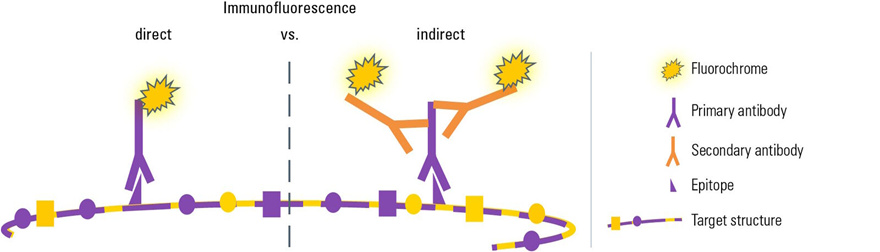
\includegraphics[width=0.91\textwidth]{abbildungen/immunoflurosenzMMV.png} % Lädt das Bild, skaliert es auf 80% der Textbreite
	\caption{ Prinzip der indirekten Immunfluoreszenz (rechts)\parencite{LeicaMicrosystems2026}} % Die Bildunterschrift
	\label{fig:immnuofMMV} % Ein Label für Querverweise (z.B. "siehe Abbildung \ref{fig:beispielbild}")
\end{figure}



Für optimale Färbungsergebnisse ist darauf zu achten, die Fixierung der
Zellen optimal sicherzustellen, geeignete Antikörper sorgfältig
auszuwählen und unspezifische Hintergrundfärbungen zu minimieren.
Letzteres wird unter anderem durch gründliche Waschschritte und
geeignete Blockierungsschritte erreicht. Zudem müssen Negativkontrollen
durchgeführt werden, um unspezifische Bindungen der Antikörper
auszuschließen. Auf diese Weise können die Auswertungen aussagekräftig
und präzise durchgeführt
werden.\footcite{LeicaIHC2026}

Um eine Kolokalisation zweier Proteine bei der mikroskopischen
Auswertung beurteilen zu können, müssen diese in einer Probe durch eine
Doppelfärbung sichtbar gemacht werden. Dazu werden zwei verschiedene,
jeweils proteinspezifische Primärantikörper eingesetzt. Dabei ist zu
beachten, dass diese aus zwei unterschiedlichen Spezies stammen. Für wissenschaftliche Zwecke werden die Antikörpern in Tieren generiert, indem sie das Antigen gespritzt bekommen, was eine gezielte Immunreaktion auslöst. Dadurch werden spezifische Antikörper produziert. Die
Sekundärantikörper sind jeweils spezifisch gegen die Spezies des
Primärantikörpers gerichtet, weshalb die Wahl von zwei
unterschiedlichen Spezies die eindeutige Zuordnung der Signale
ermöglicht und Kreuzreaktionen vermeidet. Zudem muss bei einer
Doppelfärbung beachtet werden, dass die an die Sekundärantikörper
gekoppelten Fluoreszenzfarbstoffe sich ausreichend unterscheiden, damit
es zu keiner Überlagerung der Signale kommt. Dies bedeutet, dass die
Spektren, in denen die Farbstoffe fluoreszieren, nicht stark überlappen
dürfen. Diese Spektren ergeben sich aus der jeweiligen Anregungs- und
Emissionswellenlänge.\footcite{Hackenberg}

Die Methode der indirekte Immunfluoreszenz wurde gewählt, da sie eine
Untersuchung der räumlichen Verteilung spezifischer Proteine innerhalb von
Nervenzellen ermöglicht. Dies ist für die vorliegenden Untersuchungen von
Bedeutung, da die Lokalisation von Proteinen an den synaptischen Strukturen
untersucht werden soll. Durch die Doppelfärbung von Caspr2 und den synaptischen
Markern VGlut und VGat beziehungsweise Contacin2 lässt sich feststellen, inwiefern
sich deren Signale räumlich überlagern. Auf diese Weise kann untersucht werden, ob
Caspr2 sowohl an erregenden als auch an hemmenden Synapsen lokalisiert ist und
ob Antikörper gegen Caspr2 die Kolokalisation von Caspr2 und Contacin-2
beeinflussen.

Mikroskopieverfahren 
Zur mikroskopischen Auswertung der Proben wurden die Methoden Widefield
Fluorescence Microscopy (WF) und Structured Illumination Microscopy (SIM)
angewendet.
Die Widefield Fluorescence Microscopy ist ein fluoreszenzmikroskopisches
Verfahren, bei dem das gesamte betrachtete Sichtfeld gleichzeitig mit Anregungslicht
beleuchtet wird. Dabei werden Fluorophore in der Probe durch Licht einer geeigneten
Wellenlänge angeregt. Nach der Anregung emittieren sie Licht mit einer anderen,
meist längeren Wellenlänge.
Eine zentrale Komponente der WF-Mikroskopie ist der dichroitische Spiegel (oder
Strahlteiler). Dieser befindet sich zwischen Lichtquelle und Mikroskopobjektiv und
erfüllt eine wichtige Trennfunktion. Das Anregungslicht wird vom Strahlteiler in
Richtung Probe reflektiert, während das von den Fluorophoren emittierte Licht den
Strahlteiler passieren kann. Die Eigenschaften des Strahlteilers müssen daher auf
die verwendeten Fluorophore abgestimmt sein, damit das Anregungslicht möglichst
effizient zur Probe gelangt und gleichzeitig das Fluoreszenzlicht zur Detektion
weitergeleitet wird. Das Mikroskopobjektiv wirkt zunächst als Kondensator und
fokussiert das Licht auf die Probe. Zudem sammelt es das von den Fluorophoren
ausgesendete Fluoreszenzlicht und bildet dieses auf einer Kamera ab.
\begin{figure}[h] % [h] versucht, das Bild hier zu platzieren (hier), [t] für oben, [b] für unten
	\centering % Zentriert das Bild horizontal
	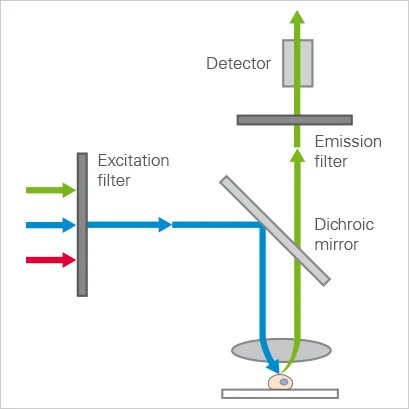
\includegraphics[width=0.91\textwidth]{abbildungen/WFMMV.jpg} % Lädt das Bild, skaliert es auf 80% der Textbreite
	\caption{ muss noch was sagen \parencite{ibidiWFMBild}} % Die Bildunterschrift
	\label{fig:WFBild} % Ein Label für Querverweise (z.B. "siehe Abbildung \ref{fig:beispielbild}")
\end{figure}
Die Structured Illumination Microscopy (SIM) ist eine Methode der
Fluoreszenzmikroskopie, mit der die Auflösung eines Lichtmikroskops verbessert
werden kann. Im Gegensatz zur WF-Mikroskopie wird die Probe nicht gleichmäßig,
sondern mit einem definierten, regelmäßigen Streifenmuster beleuchtet. Dieses
Muster entsteht durch die Interferenz von Laserstrahlen, die mithilfe eines
Beugungsgitters erzeugt werden.  
\begin{figure}[h] % [h] versucht, das Bild hier zu platzieren (hier), [t] für oben, [b] für unten
	\centering % Zentriert das Bild horizontal
	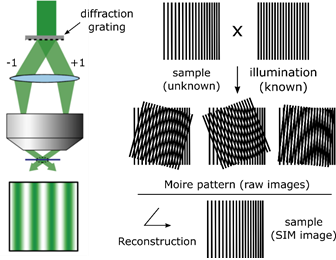
\includegraphics[width=0.91\textwidth]{abbildungen/SIMMMV.png} % Lädt das Bild, skaliert es auf 80% der Textbreite
	\caption{ muss noch was sagen \parencite{OxInstSIMBild}} % Die Bildunterschrift
	\label{fig:SIMBild} % Ein Label für Querverweise (z.B. "siehe Abbildung \ref{fig:beispielbild}")
\end{figure}
Sehr kleine Strukturen weisen hohe räumliche Frequenzen auf. Diese liegen
teilweise außerhalb des Frequenzbereichs, den das Mikroskop aufgrund seiner
begrenzten Auflösung übertragen kann. Durch die Überlagerung der hochfrequenten
Strukturen der Probe mit dem bekannten Beleuchtungsmuster entstehen jedoch
zusätzliche Frequenzanteile. Dabei wird ein Teil der ursprünglich nicht direkt
erfassbaren hochfrequenten Information in einen niedrigeren Frequenzbereich
verschoben, der vom Mikroskop detektiert werden kann. Im aufgenommenen Bild
erscheint diese Wechselwirkung zwischen dem bekannten Beleuchtungsmuster und
den Strukturen der Probe als sogenanntes Moiré-Muster.
Um möglichst viele Informationen über die Probe zu erhalten, wird das
Beleuchtungsmuster in verschiedene Richtungen gedreht und verschoben. Bei der
2D-SIM werden dafür typischerweise neun Einzelaufnahmen und bei der 3D-SIM 15
Einzelaufnahmen aufgenommen. (Haben wir 2 oder 3d gemacht?)
Anschließend werden die Einzelaufnahmen mithilfe von Softwares zu einem Bild
verarbeitet.

Neben der WF Mikroskopie wurde die SIM Mikroskopie eingesetzt, da die höhere
räumliche Auflösung der SIM Mikroskopie für die Fragestellungen der Arbeit von
Bedeutung ist. Die Wide Field Mikroskopie ermöglicht zwar eine Darstellung der
fluoreszenzmarkierten Proteine, weshalb sie sich grundsätzlich zur Untersuchung der
Proben eignet. Jedoch kommt es bei sehr kleinen oder dicht beieinander liegenden

Strukturen dazu, dass sich ihre Fluoreszenzsignale nicht eindeutig voneinander
unterscheiden lassen. Zudem findet bei der WF Mikroskopie keine optische
Schnittbildung statt, da nicht nur eine bestimmte Ebene angeregt wird, sondern auch
Fluorophore anderer Ebenen fluoreszieren. Dies ist bei der Untersuchung der
Kolokalisation zu beachten, da eine scheinbare Überlagerung von Signalen nicht
zwangsläufig einer tatsächlichen räumlichen Übereinstimmung der untersuchten
Strukturen entspricht. Durch den Einsatz der SIM Mikroskopie können die
fluoreszenzmarkierten Strukturen detaillierter dargestellt und die
Kolokalisationsflächen dadurch genauer untersucht werden. Die zusätzliche
Verwendung der Wide Field Mikroskopie ermöglicht einen größeren Überblick mit
schneller Aufnahmegeschwindigkeit über die Zellproben.\footcite{oxinstSIM}
\section{Begründung der Methodenwahl}
können wir glaub weg machen und lieber den einzelnen Methoden Kapitelchen geben evt
\section{Material}